\documentclass[11pt]{article}
\usepackage{parskip}
\parskip=1\baselineskip \advance\parskip by 0pt plus 2pt
\usepackage[pdftex]{graphicx}
\usepackage[utf8]{inputenc}
\usepackage[margin=1in]{geometry}
\usepackage{url}
\begin{document}

\begin{titlepage}
\begin{center}

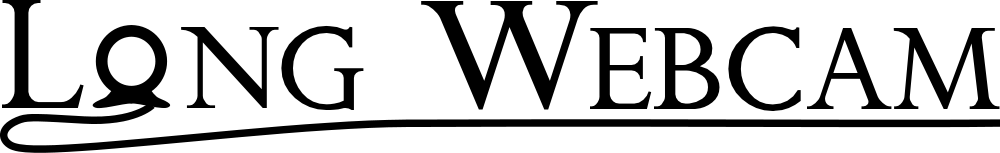
\includegraphics[width=0.85\textwidth]{./Logo_Large-cropped_black.png}

\vspace{3 cm}

\textbf{\Huge{Image Server Design}}

\vspace{1 cm}

\textit{\large{Version 1.02 - 1st July 2013}}

\vspace{4 cm}

\textbf{\Large{Authors:}}

\textbf{Steve Jones} (steve@longwebcam.org)

\end{center}

\end{titlepage}

\setcounter{tocdepth}{2}
\tableofcontents
\clearpage
\pagenumbering{roman}
\section*{Document History}
    \addcontentsline{toc}{section}{Document History}
\begin{table*}[tbhp!]
\begin{tabular}{ c c p{4in} }
\textbf{Version} & \textbf{Date} & \textbf{Notes} \\
0.10 & 5 May 2013 & Document development; The version number will be held at 0.1 until all sections have been written. \\
1.00 & 11 May 2013 & Document completed. \\
1.01 & 1 Jul 2013 & Image server will now be folded into the main Long Webcam site. Note added to introduction. \\
1.02 & 1 Jul 2013 & Added details of time zone requirements for image uploads.
\end{tabular}
\end{table*}

\clearpage
\pagenumbering{arabic}


\section{Introduction}
The Image Server will be responsible for managing all image storage and retrieval for the Long Webcam project. These are the only two functions that will be performed.

\textbf{Note:} The image server will no longer be a standalone server, but will be folded into the main Long Webcam application. Image retrieval will be accessed via \url{http://www.longwebcam.org/image/<cam_id>/<date>}, and uploads will be through \url{http://www.longwebcam.org/upload}.

\section{Data Storage}
All the images for the project will be stored in a single directory tree, whose root will be configured in the Image Server. Beneath this, each camera will have its own sub-directory (named as the camera's ID as stored in the database). All images for that camera will be stored in the directory, with a filename corresponding to the date that the image was captured (i.e. YYYYMMD.jpg). 

Performance tests have shown that this approach will not suffer a reduction in performance in retrieving images until several decades into the project.

\section{Image Upload}
The Image Server will receive images to be stored in the archive. Most of these images will be passed to the Image Server from other parts of the site. However, net-connected cameras will add images from wherever they are on the Internet, so connections must be accepted from any server. This has implications for security, in that the system must guard against images being uploaded from non-project sources. Consequently, each camera will be given a four-digit security code which must be supplied with each image.

\subsection{Upload requests}
Each upload to the image server must supply several pieces of information to allow correct storage. This includes:

\begin{itemize}
\item Camera ID
\item Camera security code
\item Image date/time
\item Image type (JPG, PNG etc.)
\item Image data
\end{itemize}

The image date and time will be in the local time zone of the camera, and will be converted to UTC with an offset as part of the data storage process.

This information will be passed to the Image Server as an XML document in a POST request. The format of the XML will be as follows:

\begin{verbatim}
<image_upload>
    <camera>
        <id>1463</id>
        <code>9656</code>
    </camera>
    <image>
        <date>20130505120000</date>
        <type>JPG</type>
        <file_data>[[Base64-encoded image file]]</file_data>
    </image>
</image_upload>
\end{verbatim}


\subsection{Upload processing}
Assuming the upload request contains the required data in the correct format, the Image Server will process the data in the following steps:

\begin{enumerate}
\item Check that the camera ID exists, and the security code matches
\item See if an image is already stored for the specified image date. If it does, raise an error. (The details of the action taken in this instance is described later.)
\item Convert the image to PNG format if required\footnote{All images will be stored in PNG format to reduce the effects of lossy compression in future processing}
\item Store the image in the camera's directory
\item Search the database for an image record for the camera and date. If it doesn't exist, create it and store the image details. If it does exist,add the image details to it.\footnote{For standalone cameras, the image records will be created every day to store weather information. The images will be provided in batches at a later date.}
\end{enumerate}

\subsection{Error handling}
There are a number of potential error conditions that can occur during a file upload. This section describes how those conditions will be handled.

\subsubsection{Malformed upload information}
If the passed in XML cannot be read, or is missing any information, this will result in an HTML return code of 400 (Bad Request). No further action will be taken.

\subsubsection{Unrecognised camera ID}
If the specified camera ID is not recognised, a 404 Not Found error will be returned

\subsubsection{Invalid security code}
If the supplied security code does not match that stored for the camera, a 403 Forbidden error will be returned.

\subsubsection{Image already exists}
If an image already exists for the specified camera and date, it is assumed that there is a problem with the client if it is supplying the same image multiple times. To help debugging, and to prevent the potential loss of project images, the uploaded XML document will be stored in a holding area for further examination. An error code of 409 (Conflict) will be returned.

\subsubsection{Bad image data}
If the encoded image data cannot be decoded into a valid image file, a 400 (Bad Request) error code will be returned. The XML request document will be stored for further examination to help with debugging.

\subsubsection{Insufficient disk space}
If there is not enough disk space on the server to store the uploaded image, a 507 (Insufficient storage) error will be returned. The client should keep the image and attempt to upload it again at a later date.

\subsection{Output}
The output of the the image upload request will be the HTTP status code (described above) and an XML document. The document will be very simple, taking the form:

\begin{verbatim}
<upload_response>
    <result>[[OK|FAIL]]</result>
    <message>[[Message]]</message>
</upload_response>
\end{verbatim}

The \verb+result+ element will contain either OK or FAIL, depending on whether or not the image was stored successfully. The \verb+message+ element will contain a short message containing the nature of the failure, or confirming successful storage.

\subsection{Signals to project administrators}
Failures to store images will be raised as system notifications against the camera concerned. However, these will not be flagged as messages that can be forwarded to the camera owner, as it is unlikely that they will be able to rectify the problem.

\section{Image retrieval}
Access to images in the archive will be through simple URLs of the form:

\begin{verbatim}
http://images.longwebcam.org/[[camera_id]]/[[date]]?[[options]]
\end{verbatim}

The URL will be taken apart to establish the image filename based on the camera ID and date. That image will be returned as the output of the request. If the image is not found, a 404 result will be returned.

Only requests from Long Webcam servers will be honoured; requests from any other server will yield a 403 Forbidden result.

\subsection{Retrieval options}
A number of options will be available to alter the returned image.

\subsubsection{size}
The size of the returned image can be requested by supplying a width and/or height of the desired image. If only one is specified, the image will be scaled to the specified size without changing the aspect ratio of the image. If both are specified, the image will be forced to that size and its aspect ratio will be ignored.

\subsubsection{watermark}
The licences for some cameras may mean that their images cannot be disseminated freely without express permission. In this case, images may be allowed if they are watermarked. The returned image will have a `destructive' watermark applied so that the image cannot be used without it being known that it came from the Long Webcam project.

\section{Interrogating the archive}
In theory, the contents of the image archive should match exactly the record of images in the site's database. However, it may be useful to interrogate the contents of the archive without having to retrieve the images themselves. Any such utility functions will be described here. As with the image retrieval function, these requests will only be accepted from the Long Webcam servers; requests from any other location will return a 403 Forbidden HTTP status code.

\end{document}

